% \title{Economic Time Series HW2}
% \author{Daeyoung Lim}

% \documentclass[answers]{exam}
\documentclass{article}
\usepackage[left=3cm,right=3cm,top=3.5cm,bottom=2cm]{geometry}
\usepackage{amssymb,amsmath,amsfonts,amsthm}
\usepackage{mathtools}
\usepackage{graphicx}
\usepackage{kotex}
\usepackage[utf8]{inputenc}
\usepackage[T1]{fontenc}
\usepackage{lmodern}
% \usepackage{enumerate}
\usepackage{listings}
\usepackage{courier}
\usepackage{cancel}
\usepackage{array}
\usepackage{courier}
\usepackage{booktabs}
\usepackage{titlesec}
\usepackage[shortlabels]{enumitem}
\usepackage{setspace}
\usepackage{newtxtext}
\usepackage[lite,nofontinfo,zswash,straightbraces]{mtpro2}
\usepackage{empheq}
\usepackage{tikz}
\usepackage{listings}

% \usepackage[toc,page]{appendix}

\setlength{\heavyrulewidth}{1.5pt}
\setlength{\abovetopsep}{4pt}

\DeclarePairedDelimiter{\ceil}{\lceil}{\rceil}
\newcommand\encircle[1]{%
  \tikz[baseline=(X.base)] 
    \node (X) [draw, shape=circle, inner sep=0] {\strut #1};}
 
% Command "alignedbox{}{}" for a box within an align environment
% Source: http://www.latex-community.org/forum/viewtopic.php?f=46&t=8144
\newlength\dlf  % Define a new measure, dlf
\newcommand\alignedbox[2]{
% Argument #1 = before & if there were no box (lhs)
% Argument #2 = after & if there were no box (rhs)
&  % Alignment sign of the line
{
\settowidth\dlf{$\displaystyle #1$}  
    % The width of \dlf is the width of the lhs, with a displaystyle font
\addtolength\dlf{\fboxsep+\fboxrule}  
    % Add to it the distance to the box, and the width of the line of the box     ㅊ
\hspace{-\dlf}  
    % Move everything dlf units to the left, so that & #1 #2 is aligned under #1 & #2
\boxed{#1 #2}
    % Put a box around lhs and rhs
}
}
\setcounter{secnumdepth}{4}
\lstset{
         basicstyle=\footnotesize\ttfamily, % Standardschrift
         %numbers=left,               % Ort der Zeilennummern
         numberstyle=\tiny,          % Stil der Zeilennummern
         %stepnumber=2,               % Abstand zwischen den Zeilennummern
         numbersep=5pt,              % Abstand der Nummern zum Text
         tabsize=2,                  % Groesse von Tabs
         extendedchars=true,         %
         breaklines=true,            % Zeilen werden Umgebrochen
         keywordstyle=\color{red},
            frame=b,         
 %        keywordstyle=[1]\textbf,    % Stil der Keywords
 %        keywordstyle=[2]\textbf,    %
 %        keywordstyle=[3]\textbf,    %
 %        keywordstyle=[4]\textbf,   \sqrt{\sqrt{}} %
         stringstyle=\color{white}\ttfamily, % Farbe der String
         showspaces=false,           % Leerzeichen anzeigen ?
         showtabs=false,             % Tabs anzeigen ?
         xleftmargin=17pt,
         framexleftmargin=17pt,
         framexrightmargin=5pt,
         framexbottommargin=4pt,
         %backgroundcolor=\color{lightgray},
         showstringspaces=false      % Leerzeichen in Strings anzeigen ?        
 }
 \lstloadlanguages{% Check Dokumentation for further languages ...
         %[Visual]Basic
         %Pascal
         %C
         %C++
         %XML
         %HTML
         Java
 }
    %\DeclareCaptionFont{blue}{\color{blue}} 

\definecolor{myblue}{RGB}{72, 165, 226}
\definecolor{myorange}{RGB}{222, 141, 8}
\titleformat{\paragraph}
{\normalfont\normalsize\bfseries}{\theparagraph}{1em}{}
\titlespacing*{\paragraph}
{0pt}{3.25ex plus 1ex minus .2ex}{1.5ex plus .2ex}
\setlength{\heavyrulewidth}{1.5pt}
\setlength{\abovetopsep}{4pt}
\setlength{\parindent}{0mm}
\linespread{1.3}
\DeclareMathOperator{\sech}{sech}
\DeclareMathOperator{\csch}{csch}
\DeclareMathOperator*{\argmin}{\arg\!\min}
\DeclareMathOperator{\tr}{tr}
\DeclareMathOperator{\ve}{vec}
% \DeclareMathOperator{\Pro}{P}

\newcommand{\bs}{\boldsymbol}
\newcommand{\opn}{\operatorname}
% \newcommand{\vecc}{\operatorname{vec}}
%%%%%%%%%%%%%%%%%%%%%%%%%%%%%%%%%%%%%%%%%%%%%%%%%%%%%%%
% % We use newtheorem to define theorem-like structures
% %
% % Here are some common ones. . .
%%%%%%%%%%%%%%%%%%%%%%%%%%%%%%%%%%%%%%%%%%%%%%%%%%%%%%%
% \newtheorem{theorem}{Theorem}
% \newtheorem{lemma}{Lemma}
% \newtheorem{proposition}{Proposition}
% \newtheorem{scolium}{Scolium}   %% And a not so common one.
% \newtheorem{definition}{Definition}
% \newenvironment{proof}{{\sc Proof:}}{~\hfill QED}
% \newenvironment{AMS}{}{}
% \newenvironment{keywords}{}{}
%%%%%%%%%%%%%%%%%%%%%%%%%%%%%%%%%%%%%%%%%%%%%%%%%%%%%%%
% %   The first thanks indicates your affiliation
% %
% %  Just the name here.
% %
% % Your mailing address goes at the end.
% %
% % \thanks is also how you indicate grant support
% %
%%%%%%%%%%%%%%%%%%%%%%%%%%%%%%%%%%%%%%%%%%%%%%%%%%%%%%%


\begin{document}
\setstretch{1.5} %줄간격 조정
\newpage
\section{HW7}
  Vector autoregression 모델을 적합하는 것은 모두 축약식에서 이루어진다. 왜냐하면 구조식에서는 model idenfication 문제가 발생하기 때문이다. 먼저 다음과 같이 일반적인 구조식을 생각해보자.
  \begin{equation}
    B_{0}y_{t} = B_{1}y_{t-1}+B_{2}y_{t-2}+\cdots + B_{p}y_{t-p}+ e_{t}
  \end{equation}
  여기서 $\mathbf{E}(e_{t})=0, \mathbf{E}(e_{t}^{}e_{t}')=I$라고 한다. 그러면 다시 다음과 같이 축약식으로 만들 수 있다.
  \begin{align}
    y_{t} &= B_{0}^{-1}B_{1}^{}y_{t-1}^{}+B_{0}^{-1}B_{2}^{}y_{t-2}^{}+\cdots+B_{0}^{-1}B_{p}^{}y_{t-p}^{} +B_{0}^{-1}e_{t}^{}\\
    &= A_{1}y_{t-1}+\cdots + A_{p}y_{t-p}+u_{t}
  \end{align}
  여기서 $B_{0}^{-1}e_{t}^{} = u_{t}$이고 $B_{0}^{-1}B_{i}^{} = A_{i}$이다. $\mathbf{E}u_{t}^{}u_{t}'=B_{0}^{-1}{B_{0}^{-1}}'=\Omega$이다. 고로 우리는 (3)번 식으로 모든 추정을 마친 뒤 추정된 $\what{\Omega}$의 Cholesky decomposition으로 $B_{0}^{-1}$을 구한 뒤 $B_{i}$들을 구하게 된다. 아직 이것만으로는 충격반응함수를 구할 수 없다. 왜냐하면 AR 표현에서 설명변수에 해당하는 $y_{t-1},\ldots,y_{t-p}$들은 서로 상관성이 있기 때문에 각각의 충격에 대해 고유한 영향을 구할 수가 없다. 이를 위해 MA 표현식으로 바꿔야 한다. 그것은 다음과 같다.
  \begin{align}
    y_{t} &= B_{0}^{-1}e_{t}^{}+\Psi_{1} B_{0}^{-1}e_{t-1}^{}+\Psi_{2}^{2}B_{0}^{-1}e_{t-2}+\cdots\\
    &= \sum_{i=0}^{\infty}\Theta_{i}e_{t-i}
  \end{align}
  위 식에서 이론적으로는 MA($\infty$)가 되지만 실제로는 무한 개의 모수를 추정하지 못하므로 lag에 따라 개수가 정해진다. 그리고 $\Psi_{i}$는 다음 블럭 행렬의 연산으로 계산된다.
  \begin{align}
    F = \begin{bmatrix}A_{1}& \cdots  &  A_{p}\\ I_{k(p-1)} & & \mathbf{0}_{k(p-1),k}  \end{bmatrix}
  \end{align}
  여기서 $\Psi_{i}=\left(F^{i}\right)_{(1,1)}$로 계산된다. Subscript $(1,1)$는 좌상단의 블럭 행렬을 가리킨다. 이제 서로 상관성이 없는 $e_{t}$들로 표현되었으니 개별적인 충격의 영향을 알 수 있게 된다.\newpage
  다음으로 충격반응함수를 보면 다음과 같다.
  \begin{center}
  \begin{figure}
  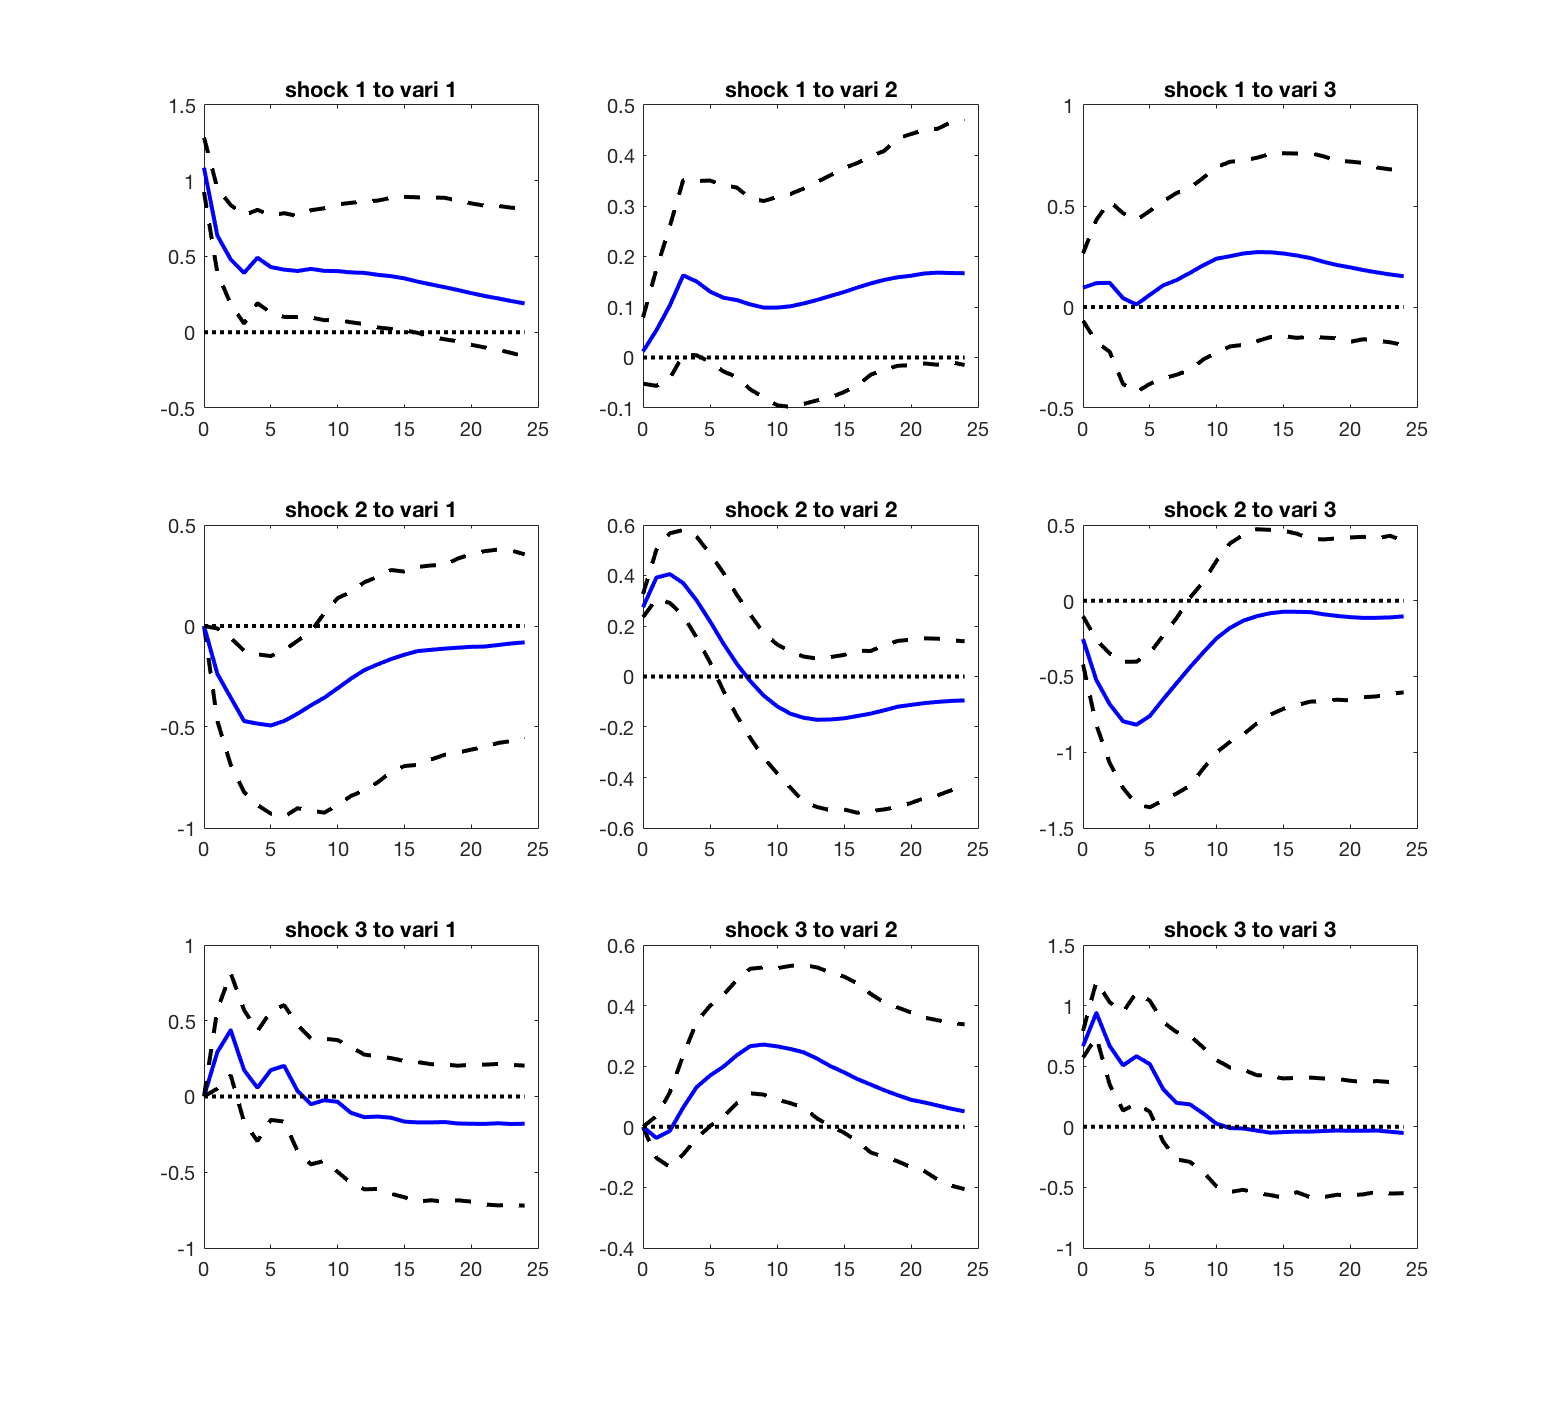
\includegraphics[scale=0.25]{before80.png}
  \caption{Before 1980}
  \end{figure}
  \end{center}
  \par
  충격반응함수는 과거의 한 단위 변화가 현재 값에 미치는 영향을 그림으로 표현한 것이므로 산점도행렬처럼 표시된 위 그래프에서 $(i,j)$ 자리의 그림은 $i$번째 변수가 $j$번째 변수에 미치는 영향을 시각화한 것이라 보면 된다. Watson 자료는 인플레이션, 실업률, 금리로 구성되어 있고 우리가 구조식에 가한 제약조건은 충격이 시간이 감에 따라 모두 0으로 갈 것이라는 가정을 반영한 것이므로 모든 그림이 0으로 수렴하고 있음을 확인할 수 있다. 인플레이션은 자기 자신과 정의 관계가 있으므로 인플레이션이 일어나면 계속해서 물가가 상승함을 의미한다. 또한 인플레이션은 금리와도 정의 상관관계를 가지고 있다.\par
  실업률은 물가와 부의 관계를 가진다. 그도 그럴 것이 실업이 일어나면 소비가 위축되고 소비가 되지 않으면 공급과잉과 함께 경기침체로 물가가 하락한다는 것이 일반적인 경제상식이다. 실업률은 금리 역시 떨어뜨린다. 왜냐하면 실업이 많아지면 중앙 은행에서는 경기를 진작시키기 위해 금리를 낮추기 때문이다.\par
  마지막으로 금리는 매우매우 외생적인 변수이다. 충격반응함수는 금리 조정이 인플레이션을 부추긴다고 그리고 있다. 또한 금리를 높이면 실업도 늘어난다.\par
  \begin{center}
  \begin{figure}
  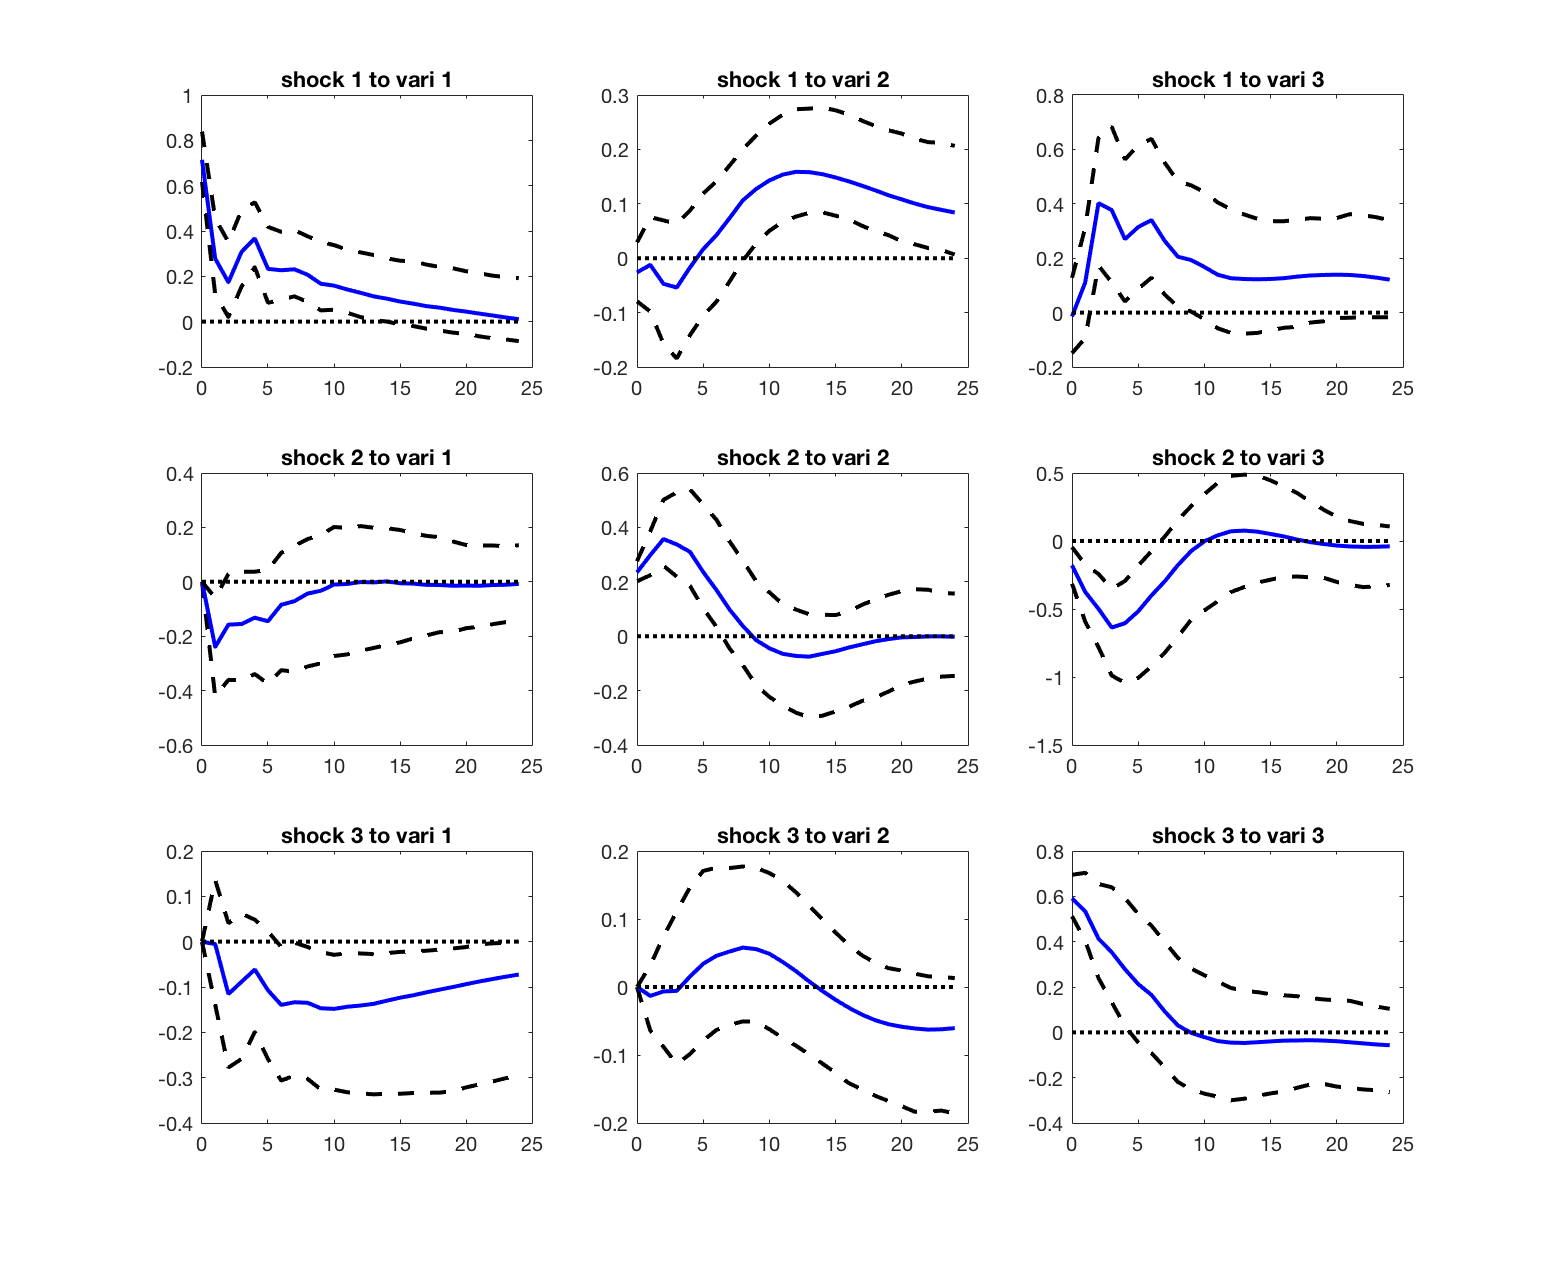
\includegraphics[scale=0.23]{after80.png}
  \caption{After 1980}
  \end{figure}
  \end{center}
  인플레이션은 실업률을 높이는 데 도움을 준다. 그리고 금리를 높이는 데도 도움을 준다. 인플레이션이 높아지면 통화량을 줄이기 위해 중앙당국에서 금리를 높일 것이기 때문이다. 실업률은 인플레이션을 낮춘다. 실업률이 높아지면 사람들이 소비를 할 수 없게 되고 그러면 경기침체로 이어져 물가가 떨어지기 때문인 것으로 보인다. 실업률은 금리를 처음에 낮췄다가 다시 조금 높이게 한다.
\end{document}
